\documentclass[conference]{IEEEtran}
\IEEEoverridecommandlockouts

\usepackage{cite}
\usepackage{amsmath,amssymb,amsfonts}
\usepackage{graphicx}
\usepackage{booktabs}
\usepackage{multirow}
\usepackage{makecell}
\usepackage{array}
\usepackage{xcolor}
\usepackage{url}
\usepackage{adjustbox}

% Paired-difference cell: mean difference on top, 95% CI below
\newcommand{\ci}[3]{\makecell{$#1$\\[-1pt]{\scriptsize[$#2$,\,$#3$]}}}

\begin{document}

\title{Disentangling Quantum Hardware Noise and Distribution Shift for Reliable Confidence Calibration in Medical Image Classification}

\author{\IEEEauthorblockN{Taye Akinrele}
\IEEEauthorblockA{\textit{Department of Computer Science}\\
\textit{The University of Alabama}\\
Tuscaloosa, Alabama, USA}}

\maketitle

% ============================================================
\begin{abstract}
Hybrid quantum--classical classifiers are being proposed for medical imaging, but a prediction is only usable clinically if its confidence is trustworthy. On noisy intermediate-scale quantum (NISQ) hardware, the scores a model produces drift with the device's noise. A deployed model can also meet a patient population whose disease rate differs from the one it was calibrated on. Both effects distort predicted probabilities. When only unlabeled deployment scores are available, they are hard to tell apart: hardware drift can look like a change in prevalence, and the reverse. We first benchmark five classifiers (a variational quantum classifier (VQC), a data re-uploading VQC, a quantum-kernel SVM, an MLP and an RBF-SVM) on MedMNIST tasks under simulated depolarizing, amplitude-damping, readout and shot noise. We find that recalibration refitted on current hardware repairs nearly all noise-induced miscalibration, whereas a calibrator frozen on calibration day does not. We then propose \emph{Shift-Disentangled Quantum Calibration} (SDQC). SDQC measures a small fixed set of probe inputs on the hardware on calibration day and again at deployment. It uses the change in their scores to map today's outputs back to the calibration-day scale, then applies a frozen Platt calibrator, and finally estimates the new disease prevalence with a shrunken expectation--maximization (EM) prior correction. Across PneumoniaMNIST, BreastMNIST and a binary OCTMNIST task, ten seeds, 29 hardware conditions (including amplitude damping never seen during design) and four target prevalences, SDQC achieves lower Brier score than frozen Platt scaling, moment matching, EM-only correction, physics-informed correction with EM, and probe correction alone in every noisy, changed-prevalence setting, with all 95\% cluster-bootstrap intervals excluding zero. On the hardest PneumoniaMNIST setting it reduces Brier from 0.0890 (frozen Platt) to 0.0446, against 0.0432 for an oracle that knows the noise and the true prevalence. The EM step has a cost when prevalence has not changed, most visibly on the small BreastMNIST set, which we report explicitly.
\end{abstract}

\begin{IEEEkeywords}
quantum machine learning, calibration, medical imaging, label shift, NISQ noise, variational quantum circuits, uncertainty quantification
\end{IEEEkeywords}

% ============================================================
\section{Introduction}

Quantum machine learning (QML) has been suggested as a route to new inductive biases for medical image analysis~\cite{sunki2025,gupta2025}. Most QML studies in this area report accuracy or AUROC. In clinical decision support, however, a model's output probability is acted on directly: a 0.9 risk score should be wrong about one time in ten. Modern neural networks are known to be miscalibrated~\cite{guo2017}, and calibration degrades further under distribution shift~\cite{ovadia2019}. Quantum classifiers add a further source of distortion. On NISQ hardware~\cite{preskill2018}, gate noise, relaxation, readout error and finite measurement shots all shrink and bias the expectation values that serve as model scores. Noise levels also drift from day to day on real devices.

This creates a specific deployment problem. A hospital calibrates a hybrid model on a labeled calibration set on a given day. Later, at deployment, two things may have changed without anyone being told: the hardware noise, and the disease prevalence among incoming patients. Only unlabeled scores are available at deployment. A shift in the score distribution could be caused by either change. Standard label-shift correction such as EM prior estimation~\cite{saerens2002} assumes the classifier itself is unchanged, so it misreads hardware drift as a change in prevalence. Conversely, matching the score distribution to the calibration-day distribution (moment matching) removes genuine changes in prevalence along with the noise. We call this the \emph{identifiability problem}: hardware drift and label shift are confounded in unlabeled data.

This paper makes three contributions:
\begin{enumerate}
\item A controlled benchmark of calibration under quantum noise for five classifiers on MedMNIST~\cite{yang2023}. It shows that miscalibration from noise is almost entirely repairable when the calibrator is refitted on current hardware, and that the practical problem is \emph{transfer}: a calibrator fitted on one day being used on another.
\item SDQC, a calibration method that separates the two effects. It uses a small fixed set of \emph{probe} inputs, measured on hardware on calibration day and at deployment, to estimate and undo hardware drift without labels. Only after that does it estimate prevalence.
\item A factorial evaluation over three datasets, three quantum models, 29 hardware conditions, four prevalences and ten seeds, with paired cluster-bootstrap confidence intervals. It reports where SDQC helps, where it costs, and how close it comes to an oracle.
\end{enumerate}
Code and results are available at \url{https://github.com/Racta-1/sdqc-quantum-calibration}.

% ============================================================
\section{Related Work}

\textbf{Calibration.} Platt scaling~\cite{platt1999}, isotonic regression~\cite{zadrozny2002} and temperature scaling~\cite{guo2017} are standard post-hoc calibrators. Niculescu-Mizil and Caruana~\cite{niculescu2005} compared them across classifier families. Ovadia et al.~\cite{ovadia2019} showed that calibration from a validation set degrades under dataset shift.

\textbf{Label shift.} Saerens et al.~\cite{saerens2002} introduced EM re-estimation of class priors from unlabeled data. Lipton et al.~\cite{lipton2018} proposed black-box shift estimation, and Alexandari et al.~\cite{alexandari2020} showed that EM works well when the underlying classifier is calibrated. All of these assume the conditional score distribution given the class, $p(z\mid y)$, is fixed. Quantum hardware drift violates that assumption.

\textbf{Quantum machine learning for imaging.} Variational quantum classifiers~\cite{schuld2020}, data re-uploading circuits~\cite{perez2020} and quantum kernel methods~\cite{havlicek2019} are the main model families. They have been applied to medical imaging using classical feature extractors to reduce dimension~\cite{gupta2025,sunki2025}. Bowles et al.~\cite{bowles2024} warn that many QML benchmarks lack fair classical baselines; we therefore include an MLP and an RBF-SVM on the same features, and a classical control that passes through the same simulated distortion.

\textbf{Uncertainty in quantum models.} Park and Simeone~\cite{park2024} studied calibrated prediction sets for quantum models with conformal prediction under shot noise and drift. Catak et al.~\cite{catak2025} and Wendlinger et al.~\cite{wendlinger2025} investigated uncertainty quantification for quantum classifiers. Spencer et al.~\cite{spencer2026} proposed adaptive calibration of quantum classifiers. To our knowledge, none of these separates hardware drift from label shift in an unlabeled deployment setting, which is the problem SDQC addresses.

% ============================================================
\section{Methodology}

\subsection{Datasets and Feature Pipeline}

We use three binary MedMNIST~\cite{yang2023} tasks at $64\times 64$ resolution (Table~\ref{tab:splits}). For OCTMNIST we construct a derived binary task, choroidal neovascularization (CNV, positive) versus NORMAL, keeping only those two classes; the pooled train and validation images are stratified-subsampled to 15,000.
Images are passed through a frozen ImageNet-pretrained ResNet-18~\cite{he2016}. The 512-dimensional embeddings are standardized and reduced to four dimensions with PCA fitted on the training split, standardized again, clipped to $\pm3$ and mapped to angles in $[0,\pi]$. The official test split is kept aside as a naturally shifted set. The remaining data are pooled and re-split into train, validation, calibration and test sets, so that calibration and in-distribution test sets share the source prevalence.

\begin{table}[t]
\centering
\caption{Data splits and positive-class prevalence (source prevalence / prevalence of the held-out shift set).}
\label{tab:splits}
\setlength{\tabcolsep}{4pt}
\begin{adjustbox}{max width=\linewidth}
\begin{tabular}{lrrrrrc}
\toprule
Dataset & Train & Val & Cal & Test & Shift & Prev. (src/shift) \\
\midrule
PneumoniaMNIST & 3138 & 524 & 785 & 785 & 624 & 0.74 / 0.62 \\
BreastMNIST    & 373  & 63  & 94  & 94  & 156 & 0.73 / 0.73 \\
OCTMNIST (bin.)& 8999 & 1501 & 2250 & 2250 & 500 & 0.42 / 0.50 \\
\bottomrule
\end{tabular}
\end{adjustbox}
\end{table}

\subsection{Classifiers}

All models act on the same four PCA features.
\begin{itemize}
\item \textbf{VQC}: four qubits, angle encoding $R_Y(x_k)$ with $x_k\in[0,\pi]$, three layers of general single-qubit rotations followed by a ring of CNOTs, readout $f=\langle Z_0\rangle$, and logit $a f + b$ (38 trainable parameters).
\item \textbf{Re-upload}: the same circuit with the data encoding repeated before each layer~\cite{perez2020}.
\item \textbf{QSVM}: a fidelity kernel from a two-repetition $R_Y/R_Z$ feature map with a CNOT chain~\cite{havlicek2019}, used in an SVC with $C=1$ trained on 600 images.
\item \textbf{MLP} (4--6--1) and \textbf{RBF-SVM}: classical baselines.
\end{itemize}
Circuits are simulated as density matrices in PennyLane~\cite{bergholm2018} (\texttt{default.mixed}). A model enters the calibration study for a given seed only if its validation AUROC is at least 0.75.

\subsection{Noise Model}

Each hardware condition $h=(p,\gamma,e_0,e_1,S)$ specifies the following. Depolarizing noise with probability $p$ is applied after every gate. Amplitude damping with rate $\gamma$ is applied after every gate. Asymmetric readout error ($e_0$: $0\!\to\!1$, $e_1$: $1\!\to\!0$) is applied analytically to the measured expectation. Finally, the score is estimated from $S$ shots by binomial sampling. For the QSVM, noise acts on the kernel estimates, which are clipped to $[0,1]$. The reference calibration-day condition is $\mathrm{REF}=(p{=}0.002,\gamma{=}0,e_0{=}e_1{=}0.02,S{=}1000)$.

\subsection{Calibration Under Known Hardware}

Let $z$ be the noisy score observed on hardware $h$. If labeled data were available on $h$ itself, one would fit Platt scaling $\hat p=\sigma(\alpha z+\beta)$ directly on $h$. We call this the \emph{Oracle Platt} calibrator. In deployment, only a calibrator fitted on REF, called \emph{Fixed Platt}, is available. The gap between the two measures how much miscalibration comes from transfer rather than from noise as such.

\subsection{Baselines for Unlabeled Deployment}

\begin{itemize}
\item \textbf{Fixed Platt}: the REF calibrator applied unchanged.
\item \textbf{Moment matching (MM)}: an affine map of today's score batch so its mean and standard deviation match the calibration-day scores, followed by Fixed Platt.
\item \textbf{EM only}: Fixed Platt followed by EM prior re-estimation~\cite{saerens2002}.
\item \textbf{Physics-informed + EM}: a parametric device-response model, fitted on a simulated grid of depolarizing and readout noise levels, maps scores back using the \emph{reported} device error rates; a noise-free Platt calibrator and EM follow. Reported rates carry a multiplicative error $\exp(\mathcal N(0,0.2^2))$, and $\gamma$ is never reported.
\item \textbf{Oracle (noise + true prior)}: Oracle Platt fitted on $h$, followed by exact prior adjustment to the true target prevalence. This is a lower bound that no deployable method can reach.
\end{itemize}

\subsection{Shift-Disentangled Quantum Calibration (SDQC)}

Fig.~\ref{fig:method} summarizes SDQC. The key observation is that drift in hardware noise changes the score of \emph{every} input in a largely systematic way. A change in prevalence, on the other hand, changes \emph{which} inputs arrive, not their individual scores. If the same fixed inputs are measured on calibration day and at deployment, any change in their scores must come from the hardware. These inputs are the \emph{probes}.

\begin{figure*}[t]
\centering
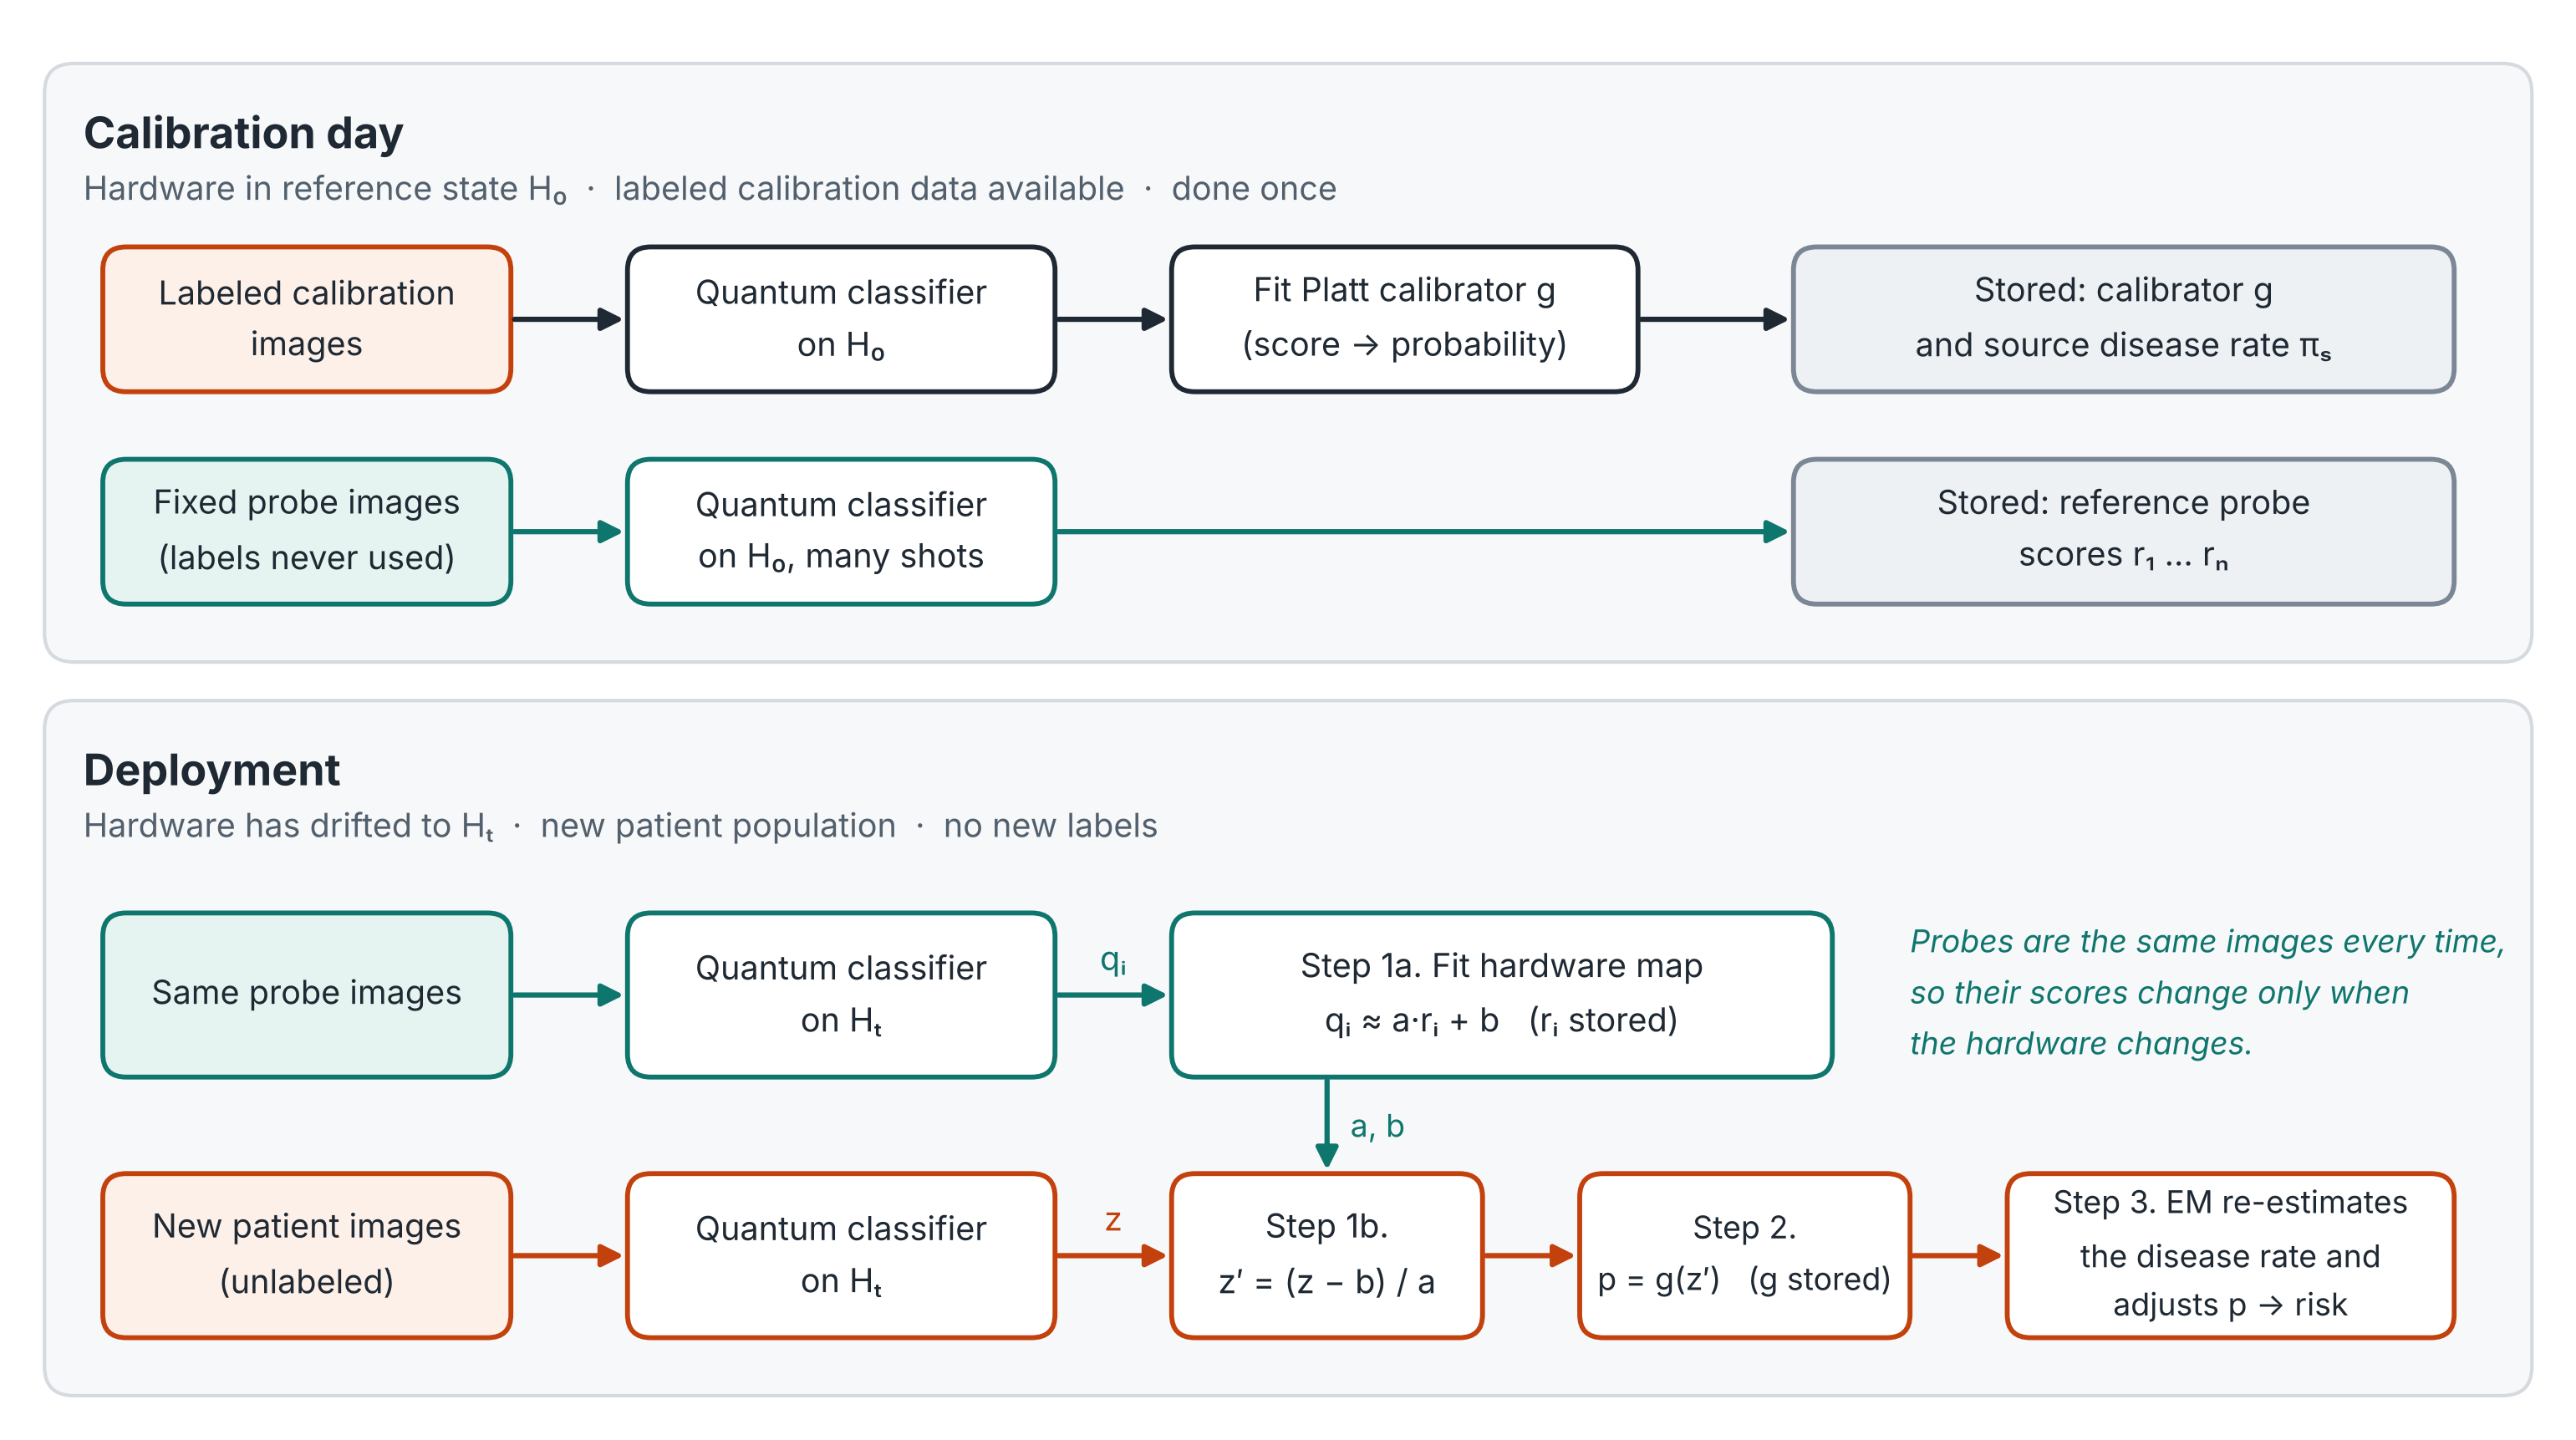
\includegraphics[width=0.92\textwidth]{sdqc_methodology.png}
\caption{SDQC pipeline. \textbf{Calibration day:} fit a Platt calibrator on labeled calibration data under the reference hardware, and record the hardware scores $r_j$ of $K$ fixed probe inputs with a high shot budget. \textbf{Deployment:} re-measure the same probes ($q_j$), fit an affine drift map, map patient scores back to the calibration-day scale, apply the frozen calibrator, and estimate the new prevalence with shrunken EM.}
\label{fig:method}
\end{figure*}

\textbf{Step 1: Calibration-day reference.} Draw $K=96$ probe inputs uniformly at random (fixed seed) from the validation split. Measure their scores on the reference hardware with $S_{\mathrm{ref}}=10{,}000$ shots to obtain $r_1,\dots,r_K$. Fit Fixed Platt $(\alpha,\beta)$ on the labeled calibration set under REF. The source prevalence is $\pi_s$.

\textbf{Step 2: Drift estimation at deployment.} Re-measure the same probes on today's hardware to obtain $q_1,\dots,q_K$. Fit the affine response
\begin{equation}
(\hat a,\hat b)=\arg\min_{a,b}\sum_{j=1}^{K}\left(q_j-a\,r_j-b\right)^2,\quad \hat a\leftarrow\mathrm{clip}(\hat a,0.1,5),
\end{equation}
and re-centre the intercept after clipping, $\hat b=\bar q-\hat a\,\bar r$.

\textbf{Step 3: Score correction and calibration.} For each patient score $z_i$,
\begin{equation}
\tilde z_i=\frac{z_i-\hat b}{\hat a},\qquad p_i=\sigma(\alpha\,\tilde z_i+\beta).
\end{equation}
Using only Steps 1--3 gives the \emph{SDQC (probe only)} ablation.

\textbf{Step 4: Prevalence estimation.} Starting from $\pi^{(0)}=\pi_s$, iterate
\begin{equation}
w_i^{(t)}=\frac{\frac{\pi^{(t)}}{\pi_s}p_i}{\frac{\pi^{(t)}}{\pi_s}p_i+\frac{1-\pi^{(t)}}{1-\pi_s}(1-p_i)},\qquad
\pi^{(t+1)}=\frac1N\sum_{i=1}^N w_i^{(t)},
\end{equation}
until convergence, giving $\pi_{\mathrm{EM}}$. Shrink it toward the source prevalence:
\begin{equation}
\hat\pi=\lambda\,\pi_{\mathrm{EM}}+(1-\lambda)\,\pi_s,\qquad \lambda=0.85.
\end{equation}
Output the prior-adjusted posterior
\begin{equation}
\hat p_i=\frac{\frac{\hat\pi}{\pi_s}p_i}{\frac{\hat\pi}{\pi_s}p_i+\frac{1-\hat\pi}{1-\pi_s}(1-p_i)}.
\end{equation}

\textbf{SDQC-sim ablation.} To test whether the reference must be measured on hardware, SDQC-sim replaces $r_j$ with noiseless simulator scores of the probes and uses a Platt calibrator fitted on noiseless calibration scores.

\textbf{Cost.} At deployment, SDQC needs $K$ extra circuit evaluations per recalibration and no labels. Probes are not patient data, so they can be stored and re-run at any time.

% ============================================================
\section{Experimental Design}

\subsection{Initial Benchmark (V4)}

The first experiment uses PneumoniaMNIST and BreastMNIST with 3 seeds. Part~A sweeps each noise type separately and compares Oracle Platt, temperature scaling and isotonic regression. Part~B measures transfer from REF to held-out depolarizing and amplitude-damping hardware for Fixed Platt, noise-conditioned Platt (NC), physics-informed correction (Phys), MM and Oracle Platt. Part~C adds label shift. Part~D varies the MM batch size.

\subsection{Main SDQC Evaluation (V5.1)}

The main study is a full factorial design:
\begin{itemize}
\item \textbf{Datasets}: PneumoniaMNIST, BreastMNIST, OCTMNIST (binary).
\item \textbf{Models}: VQC, Re-upload and QSVM, each included for a seed only if it passes the AUROC gate. BreastMNIST QSVM never passes; BreastMNIST Re-upload passes in 8 of 10 seeds.
\item \textbf{Hardware}, 29 conditions per model and seed:
  \begin{itemize}
  \item \emph{clean}: REF itself;
  \item \emph{held-out depolarizing} (20): $p\in\{0.001,0.005,0.015,0.02,0.05\}$, each crossed with 4 random readout settings $e_0,e_1\in[0,0.08]$;
  \item \emph{unseen amplitude damping} (8): $\gamma\in\{0.01,0.03\}$ on top of $p=0.002$, each crossed with 4 readout settings.
  \end{itemize}
  All conditions use 1,000 shots. Amplitude damping was never used to design or tune any method.
\item \textbf{Target prevalence}: the source prevalence (\emph{same}) or $\pi_t\in\{0.30,0.50,0.90\}$ (\emph{changed}). Each changed prevalence is obtained by subsampling the test set without replacement.
\item \textbf{Seeds}: 10 (0--9).
\end{itemize}

\textbf{Metrics.} The primary metric is the Brier score. Secondary metrics are negative log-likelihood (NLL), expected calibration error (ECE, 15 equal-width bins), AUROC and the absolute error of the estimated prevalence. Differences between methods are paired within the same seed $\times$ model $\times$ hardware condition $\times$ prevalence. 95\% confidence intervals come from a cluster bootstrap (2,000 resamples) over seed $\times$ model $\times$ hardware-condition clusters. A difference is reported as \emph{SDQC minus comparator}, so negative values favour SDQC.

% ============================================================
\section{Results}

\subsection{Model Sanity}

Table~\ref{tab:sanity} reports discrimination. On PneumoniaMNIST and OCTMNIST all five models reach AUROC of about 0.97--0.98, so quantum and classical models discriminate equally well on these features. On BreastMNIST, QSVM (mean validation AUROC 0.738) and RBF-SVM (0.714) fail the 0.75 gate and are excluded from the calibration study.

\begin{table}[t]
\centering
\caption{Mean validation / test AUROC under the reference hardware (V5.1, 10 seeds). $^\dagger$Excluded by the 0.75 validation-AUROC gate in every seed. $^\ddagger$Passes the gate in 8 of 10 seeds.}
\label{tab:sanity}
\setlength{\tabcolsep}{4pt}
\begin{adjustbox}{max width=\linewidth}
\begin{tabular}{lccc}
\toprule
Model & PneumoniaMNIST & BreastMNIST & OCTMNIST \\
\midrule
VQC       & 0.978 / 0.983 & 0.781 / 0.828 & 0.975 / 0.974 \\
Re-upload & 0.977 / 0.981 & 0.769 / 0.848$^\ddagger$ & 0.975 / 0.973 \\
QSVM      & 0.972 / 0.977 & 0.738 / 0.839$^\dagger$ & 0.972 / 0.969 \\
MLP       & 0.977 / 0.981 & 0.785 / 0.835 & 0.977 / 0.974 \\
RBF-SVM   & 0.970 / 0.982 & 0.714 / 0.848$^\dagger$ & 0.977 / 0.973 \\
\bottomrule
\end{tabular}
\end{adjustbox}
\end{table}

\subsection{Initial Benchmark: Noise Is Repairable, Transfer Is Not}

\textbf{Part A (in-place recalibration).} When Platt scaling is refitted on the same hardware, the extra Brier score caused by noise is at most $0.0006$ for every model and noise type. Temperature scaling leaves $+0.036$ to $+0.093$ Brier at the strongest noise levels, because noise biases the scores as well as shrinking them, and one temperature cannot correct a shift. Shot noise down to 100 shots costs about $+0.004$. Noise therefore damages calibration, but in a way that is easy to repair \emph{if} labeled data on the current hardware exist.

\textbf{Part B (transfer).} Table~\ref{tab:v4b} and Fig.~\ref{fig:v4b} show that a calibrator frozen on REF is clearly worse than Oracle Platt. For example, on VQC with depolarizing noise, Brier rises from 0.054 to 0.069. Moment matching nearly closes the gap when prevalence is unchanged, as do physics-informed correction and, to a lesser degree, NC. The classical control behaves in the same way as the quantum models, which shows that the effect comes from the distortion, not from anything specifically quantum.

\begin{table}[t]
\centering
\caption{V4 Part B: mean Brier when transferring a REF calibrator to held-out hardware (PneumoniaMNIST, 3 seeds, source prevalence). NC: noise-conditioned Platt; Phys: physics-informed; MM: moment matching.}
\label{tab:v4b}
\setlength{\tabcolsep}{4pt}
\begin{adjustbox}{max width=\linewidth}
\begin{tabular}{llccccc}
\toprule
Model & Noise & Fixed & NC & Phys & MM & Oracle \\
\midrule
\multirow{2}{*}{VQC}       & Depol. & 0.069 & 0.059 & 0.055 & 0.055 & 0.054 \\
                           & Amp.   & 0.058 & 0.055 & 0.055 & 0.049 & 0.049 \\
\multirow{2}{*}{Re-upload} & Depol. & 0.079 & 0.067 & 0.063 & 0.061 & 0.060 \\
                           & Amp.   & 0.064 & 0.061 & 0.062 & 0.051 & 0.051 \\
\multirow{2}{*}{QSVM}      & Depol. & 0.077 & 0.061 & 0.061 & 0.061 & 0.060 \\
                           & Amp.   & 0.061 & 0.060 & 0.060 & 0.053 & 0.053 \\
\multirow{2}{*}{Control}   & Depol. & 0.071 & 0.060 & 0.057 & 0.056 & 0.056 \\
                           & Amp.   & 0.061 & 0.058 & 0.058 & 0.050 & 0.050 \\
\bottomrule
\end{tabular}
\end{adjustbox}
\end{table}

\begin{figure*}[t]
\centering
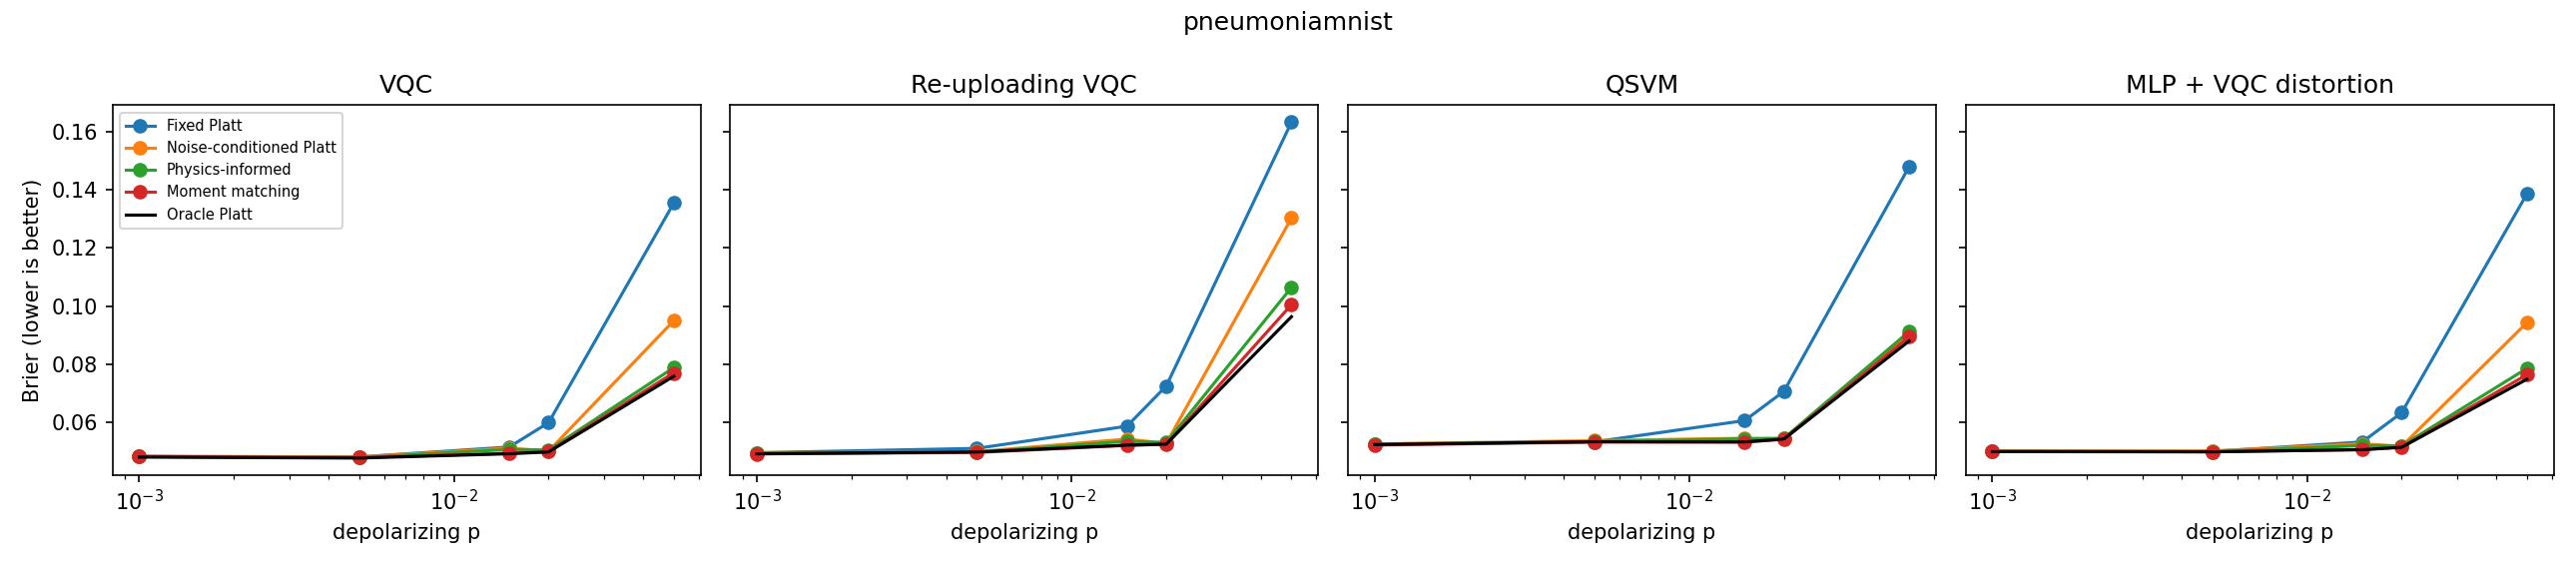
\includegraphics[width=\textwidth]{v4_partB_pneumoniamnist.png}
\caption{V4 Part B on PneumoniaMNIST: Brier score of each transfer method as depolarizing noise $p$ increases, for each model (REF calibrator, source prevalence).}
\label{fig:v4b}
\end{figure*}

\textbf{Part C (adding label shift).} Table~\ref{tab:v4c} shows the identifiability problem directly. Once prevalence changes, MM becomes the \emph{worst} method (0.167--0.175), because it removes the genuine change in prevalence along with the noise. Physics-informed correction followed by EM comes close to the oracle, but it relies on device error reports that are accurate in this experiment. That motivates a method that needs no such reports.

\begin{table}[t]
\centering
\caption{V4 Part C: mean Brier over shifted target prevalences.}
\label{tab:v4c}
\setlength{\tabcolsep}{3.5pt}
\begin{adjustbox}{max width=\linewidth}
\begin{tabular}{lcccccc}
\toprule
Hardware & Fixed & Phys & Phys+EM & MM & MM+EM & Oracle \\
\midrule
No noise & 0.062 & 0.062 & 0.046 & 0.167 & 0.144 & 0.046 \\
Noise    & 0.089 & 0.064 & 0.050 & 0.175 & 0.153 & 0.049 \\
\bottomrule
\end{tabular}
\end{adjustbox}
\end{table}

\textbf{Part D (MM batch size).} MM needs a large deployment batch: Brier is 0.067 at 16 samples, 0.059 at 32, 0.056 at 64, 0.055 at 128 and 0.054 using all samples (Table~\ref{tab:v4d}).

\begin{table}[t]
\centering
\caption{V4 Part D: moment-matching Brier versus deployment batch size.}
\label{tab:v4d}
\begin{adjustbox}{max width=\linewidth}
\begin{tabular}{lccccc}
\toprule
Batch size & 16 & 32 & 64 & 128 & All \\
\midrule
Brier & 0.067 & 0.059 & 0.056 & 0.055 & 0.054 \\
\bottomrule
\end{tabular}
\end{adjustbox}
\end{table}

\subsection{Main Result: SDQC Across Datasets, Noise and Prevalence}

Table~\ref{tab:brier} gives the full mean Brier results. Three patterns are clear.

\emph{(i) Changed prevalence with noise.} This is the target setting. In all six dataset $\times$ noise-family cells, SDQC has lower Brier than every baseline (Fixed, MM, EM only, Phys+EM and probe only). It is within 0.0003 of SDQC-sim and within 0.0014--0.0130 of the oracle.

\emph{(ii) Unseen amplitude damping.} Physics-informed correction depends on noise types it knows, so it degrades. On BreastMNIST it scores 0.1950, against 0.1370 for SDQC. Probes measure the actual hardware response whatever its physical cause, so SDQC transfers.

\emph{(iii) Same prevalence.} SDQC matches the oracle closely on PneumoniaMNIST and OCTMNIST. On BreastMNIST its EM step costs about $0.012$--$0.015$ Brier compared with probe-only correction. EM-only is badly unstable there (0.3172 under depolarizing noise).

\begin{table*}[t]
\centering
\caption{Mean Brier score (V5.1; 10 seeds; models passing the AUROC gate; averaged over hardware conditions in each family and over target prevalences). \emph{Changed}: $\pi_t\in\{0.30,0.50,0.90\}$; \emph{same}: source prevalence. Lowest Brier among methods other than the oracle in bold.}
\label{tab:brier}
\setlength{\tabcolsep}{4.5pt}
\begin{adjustbox}{max width=\linewidth}
\begin{tabular}{lllcccccccc}
\toprule
Dataset & Hardware & Prev. & Fixed & MM & EM only & Phys+EM & Probe only & SDQC-sim & SDQC & Oracle \\
\midrule
\multirow{6}{*}{BreastMNIST}
 & Clean        & changed & 0.1660 & 0.2263 & \textbf{0.1349} & 0.1387 & 0.1667 & 0.1387 & 0.1386 & 0.1300 \\
 & Clean        & same    & 0.1264 & \textbf{0.1259} & 0.1324 & 0.1368 & 0.1269 & 0.1368 & 0.1366 & 0.1270 \\
 & Depolarizing & changed & 0.1881 & 0.2286 & 0.2556 & 0.1572 & 0.1728 & \textbf{0.1434} & \textbf{0.1434} & 0.1304 \\
 & Depolarizing & same    & 0.1466 & \textbf{0.1332} & 0.3172 & 0.1693 & 0.1370 & 0.1516 & 0.1516 & 0.1347 \\
 & Amp. damping & changed & 0.1820 & 0.2250 & 0.2367 & 0.1950 & 0.1665 & 0.1373 & \textbf{0.1370} & 0.1282 \\
 & Amp. damping & same    & 0.1409 & \textbf{0.1283} & 0.2828 & 0.2164 & 0.1297 & 0.1416 & 0.1413 & 0.1298 \\
\midrule
\multirow{6}{*}{OCTMNIST}
 & Clean        & changed & 0.0661 & 0.1398 & 0.0534 & 0.0517 & 0.0651 & 0.0517 & \textbf{0.0516} & 0.0499 \\
 & Clean        & same    & 0.0590 & \textbf{0.0585} & 0.0591 & 0.0586 & \textbf{0.0585} & 0.0586 & \textbf{0.0585} & 0.0586 \\
 & Depolarizing & changed & 0.0943 & 0.1537 & 0.1271 & 0.0704 & 0.0801 & \textbf{0.0661} & 0.0662 & 0.0605 \\
 & Depolarizing & same    & 0.0961 & \textbf{0.0728} & 0.1617 & 0.0778 & 0.0737 & 0.0738 & 0.0739 & 0.0714 \\
 & Amp. damping & changed & 0.0742 & 0.1431 & 0.0721 & 0.0662 & 0.0682 & 0.0548 & \textbf{0.0547} & 0.0525 \\
 & Amp. damping & same    & 0.0708 & \textbf{0.0620} & 0.0879 & 0.0801 & \textbf{0.0620} & 0.0621 & \textbf{0.0620} & 0.0619 \\
\midrule
\multirow{6}{*}{PneumoniaMNIST}
 & Clean        & changed & 0.0594 & 0.1686 & 0.0447 & \textbf{0.0439} & 0.0603 & \textbf{0.0439} & \textbf{0.0439} & 0.0428 \\
 & Clean        & same    & 0.0502 & \textbf{0.0495} & 0.0502 & 0.0496 & \textbf{0.0495} & 0.0496 & \textbf{0.0495} & 0.0496 \\
 & Depolarizing & changed & 0.1084 & 0.1810 & 0.1061 & 0.0587 & 0.0728 & \textbf{0.0552} & 0.0553 & 0.0518 \\
 & Depolarizing & same    & 0.0760 & \textbf{0.0589} & 0.1047 & 0.0629 & 0.0596 & 0.0596 & 0.0598 & 0.0584 \\
 & Amp. damping & changed & 0.0890 & 0.1719 & 0.0650 & 0.0613 & 0.0621 & 0.0447 & \textbf{0.0446} & 0.0432 \\
 & Amp. damping & same    & 0.0622 & \textbf{0.0512} & 0.0791 & 0.0786 & 0.0513 & 0.0514 & 0.0513 & 0.0512 \\
\bottomrule
\end{tabular}
\end{adjustbox}
\end{table*}

\subsection{Paired Comparisons}

Table~\ref{tab:paired_changed} gives paired differences with 95\% confidence intervals for the changed-prevalence setting. Against every deployable baseline (Fixed, MM, EM only, Phys+EM and probe only), SDQC is better in all six cells, and every interval excludes zero. The improvement over Phys+EM is small under depolarizing noise ($-0.0034$ to $-0.0138$), because Phys+EM was designed for that noise type. It is much larger under unseen amplitude damping ($-0.0114$ to $-0.0580$). SDQC and SDQC-sim differ by at most 0.0003 Brier. The oracle remains better by 0.0014--0.0130.

\begin{table*}[t]
\centering
\caption{Paired Brier difference, SDQC minus comparator, with 95\% cluster-bootstrap CI (10 seeds): \textbf{changed prevalence}. Negative values favour SDQC.}
\label{tab:paired_changed}
\setlength{\tabcolsep}{3pt}
\renewcommand{\arraystretch}{1.25}
\begin{adjustbox}{max width=\linewidth}
\begin{tabular}{llccccccc}
\toprule
Dataset & Hardware & vs Fixed & vs MM & vs EM only & vs Phys+EM & vs Probe only & vs SDQC-sim & vs Oracle \\
\midrule
\multirow{2}{*}{Pneumonia}
 & Depol. & \ci{-0.0531}{-0.0573}{-0.0493} & \ci{-0.1257}{-0.1266}{-0.1247} & \ci{-0.0508}{-0.0588}{-0.0431} & \ci{-0.0034}{-0.0044}{-0.0025} & \ci{-0.0175}{-0.0177}{-0.0173} & \ci{+0.0000}{-0.0000}{0.0001} & \ci{+0.0034}{0.0030}{0.0039} \\
 & Amp. & \ci{-0.0444}{-0.0483}{-0.0407} & \ci{-0.1273}{-0.1286}{-0.1260} & \ci{-0.0204}{-0.0256}{-0.0158} & \ci{-0.0167}{-0.0192}{-0.0142} & \ci{-0.0175}{-0.0177}{-0.0172} & \ci{-0.0001}{-0.0001}{-0.0001} & \ci{+0.0014}{0.0013}{0.0015} \\
\midrule
\multirow{2}{*}{OCT}
 & Depol. & \ci{-0.0280}{-0.0302}{-0.0261} & \ci{-0.0874}{-0.0880}{-0.0869} & \ci{-0.0608}{-0.0688}{-0.0534} & \ci{-0.0042}{-0.0057}{-0.0029} & \ci{-0.0139}{-0.0140}{-0.0138} & \ci{+0.0001}{0.0000}{0.0002} & \ci{+0.0057}{0.0050}{0.0065} \\
 & Amp. & \ci{-0.0195}{-0.0208}{-0.0183} & \ci{-0.0884}{-0.0893}{-0.0875} & \ci{-0.0174}{-0.0241}{-0.0117} & \ci{-0.0114}{-0.0154}{-0.0080} & \ci{-0.0135}{-0.0136}{-0.0134} & \ci{-0.0001}{-0.0001}{-0.0001} & \ci{+0.0022}{0.0021}{0.0022} \\
\midrule
\multirow{2}{*}{Breast}
 & Depol. & \ci{-0.0447}{-0.0469}{-0.0426} & \ci{-0.0852}{-0.0869}{-0.0833} & \ci{-0.1122}{-0.1246}{-0.1002} & \ci{-0.0138}{-0.0183}{-0.0096} & \ci{-0.0294}{-0.0308}{-0.0280} & \ci{-0.0000}{-0.0003}{0.0003} & \ci{+0.0130}{0.0113}{0.0148} \\
 & Amp. & \ci{-0.0449}{-0.0480}{-0.0420} & \ci{-0.0880}{-0.0896}{-0.0864} & \ci{-0.0996}{-0.1162}{-0.0849} & \ci{-0.0580}{-0.0715}{-0.0460} & \ci{-0.0294}{-0.0311}{-0.0277} & \ci{-0.0003}{-0.0007}{0.0002} & \ci{+0.0089}{0.0078}{0.0100} \\
\bottomrule
\end{tabular}
\end{adjustbox}
\end{table*}

Table~\ref{tab:paired_same} gives the same comparisons when prevalence has \emph{not} changed. Here the EM step can only add noise. On PneumoniaMNIST and OCTMNIST the cost is negligible: compared with MM and probe-only correction it is at most $+0.0011$. SDQC still improves on Fixed Platt, EM-only and Phys+EM. On BreastMNIST, with only 94 test images, the cost is real: $+0.0146$ (depolarizing) and $+0.0117$ (amplitude damping) compared with probe-only correction. Against Fixed Platt, SDQC is worse under depolarizing noise ($+0.0051$) and shows no clear difference under amplitude damping ($+0.0004$).

\begin{table*}[t]
\centering
\caption{Paired Brier difference, SDQC minus comparator, with 95\% cluster-bootstrap CI (10 seeds): \textbf{same (source) prevalence}. Negative values favour SDQC.}
\label{tab:paired_same}
\setlength{\tabcolsep}{3pt}
\renewcommand{\arraystretch}{1.25}
\begin{adjustbox}{max width=\linewidth}
\begin{tabular}{llccccccc}
\toprule
Dataset & Hardware & vs Fixed & vs MM & vs EM only & vs Phys+EM & vs Probe only & vs SDQC-sim & vs Oracle \\
\midrule
\multirow{2}{*}{Pneumonia}
 & Depol. & \ci{-0.0162}{-0.0181}{-0.0144} & \ci{+0.0010}{0.0008}{0.0012} & \ci{-0.0449}{-0.0517}{-0.0385} & \ci{-0.0030}{-0.0042}{-0.0020} & \ci{+0.0002}{0.0002}{0.0003} & \ci{+0.0002}{0.0001}{0.0003} & \ci{+0.0015}{0.0012}{0.0018} \\
 & Amp. & \ci{-0.0109}{-0.0128}{-0.0090} & \ci{+0.0002}{0.0001}{0.0002} & \ci{-0.0277}{-0.0332}{-0.0228} & \ci{-0.0273}{-0.0317}{-0.0231} & \ci{+0.0000}{0.0000}{0.0001} & \ci{-0.0000}{-0.0000}{-0.0000} & \ci{+0.0001}{0.0001}{0.0002} \\
\midrule
\multirow{2}{*}{OCT}
 & Depol. & \ci{-0.0221}{-0.0252}{-0.0193} & \ci{+0.0011}{0.0009}{0.0014} & \ci{-0.0878}{-0.0994}{-0.0762} & \ci{-0.0039}{-0.0057}{-0.0025} & \ci{+0.0003}{0.0002}{0.0003} & \ci{+0.0001}{0.0000}{0.0002} & \ci{+0.0025}{0.0020}{0.0030} \\
 & Amp. & \ci{-0.0087}{-0.0109}{-0.0070} & \ci{+0.0000}{0.0000}{0.0001} & \ci{-0.0259}{-0.0351}{-0.0180} & \ci{-0.0180}{-0.0242}{-0.0130} & \ci{+0.0000}{0.0000}{0.0000} & \ci{-0.0000}{-0.0001}{-0.0000} & \ci{+0.0002}{0.0001}{0.0002} \\
\midrule
\multirow{2}{*}{Breast}
 & Depol. & \ci{+0.0051}{0.0029}{0.0074} & \ci{+0.0184}{0.0164}{0.0206} & \ci{-0.1656}{-0.1841}{-0.1473} & \ci{-0.0177}{-0.0250}{-0.0114} & \ci{+0.0146}{0.0132}{0.0161} & \ci{+0.0000}{-0.0003}{0.0004} & \ci{+0.0169}{0.0150}{0.0191} \\
 & Amp. & \ci{+0.0004}{-0.0013}{0.0020} & \ci{+0.0130}{0.0117}{0.0144} & \ci{-0.1415}{-0.1662}{-0.1169} & \ci{-0.0751}{-0.0965}{-0.0568} & \ci{+0.0117}{0.0105}{0.0129} & \ci{-0.0003}{-0.0007}{0.0002} & \ci{+0.0115}{0.0103}{0.0128} \\
\bottomrule
\end{tabular}
\end{adjustbox}
\end{table*}

\subsection{The Hard Case: Unseen Noise and Changed Prevalence}

Table~\ref{tab:hard} reports NLL and ECE for the hardest setting, unseen amplitude damping with changed prevalence. The ranking matches the Brier results. On OCTMNIST and PneumoniaMNIST, SDQC cuts ECE from 0.095 and 0.136 (Fixed Platt) to 0.027 and 0.037, close to the oracle's 0.020 and 0.035. Fig.~\ref{fig:hard} shows this setting visually.

\begin{table*}[t]
\centering
\caption{Hard case (unseen amplitude damping, changed prevalence): mean NLL and ECE (15 bins), 10 seeds. Lowest among methods other than the oracle in bold.}
\label{tab:hard}
\setlength{\tabcolsep}{4.5pt}
\begin{adjustbox}{max width=\linewidth}
\begin{tabular}{llcccccccc}
\toprule
Dataset & Metric & Fixed & MM & EM only & Phys+EM & Probe only & SDQC-sim & SDQC & Oracle \\
\midrule
\multirow{2}{*}{BreastMNIST}
 & NLL & 0.549 & 0.683 & 0.699 & 0.583 & 0.521 & 0.427 & \textbf{0.426} & 0.402 \\
 & ECE & 0.236 & 0.288 & 0.270 & 0.222 & 0.213 & \textbf{0.163} & \textbf{0.163} & 0.139 \\
\midrule
\multirow{2}{*}{OCTMNIST}
 & NLL & 0.255 & 0.579 & 0.241 & 0.221 & 0.236 & 0.189 & \textbf{0.188} & 0.181 \\
 & ECE & 0.095 & 0.167 & 0.071 & 0.061 & 0.058 & 0.028 & \textbf{0.027} & 0.020 \\
\midrule
\multirow{2}{*}{PneumoniaMNIST}
 & NLL & 0.280 & 0.590 & 0.219 & 0.206 & 0.202 & \textbf{0.153} & \textbf{0.153} & 0.150 \\
 & ECE & 0.136 & 0.232 & 0.086 & 0.083 & 0.072 & \textbf{0.037} & \textbf{0.037} & 0.035 \\
\bottomrule
\end{tabular}
\end{adjustbox}
\end{table*}

\begin{figure*}[t]
\centering
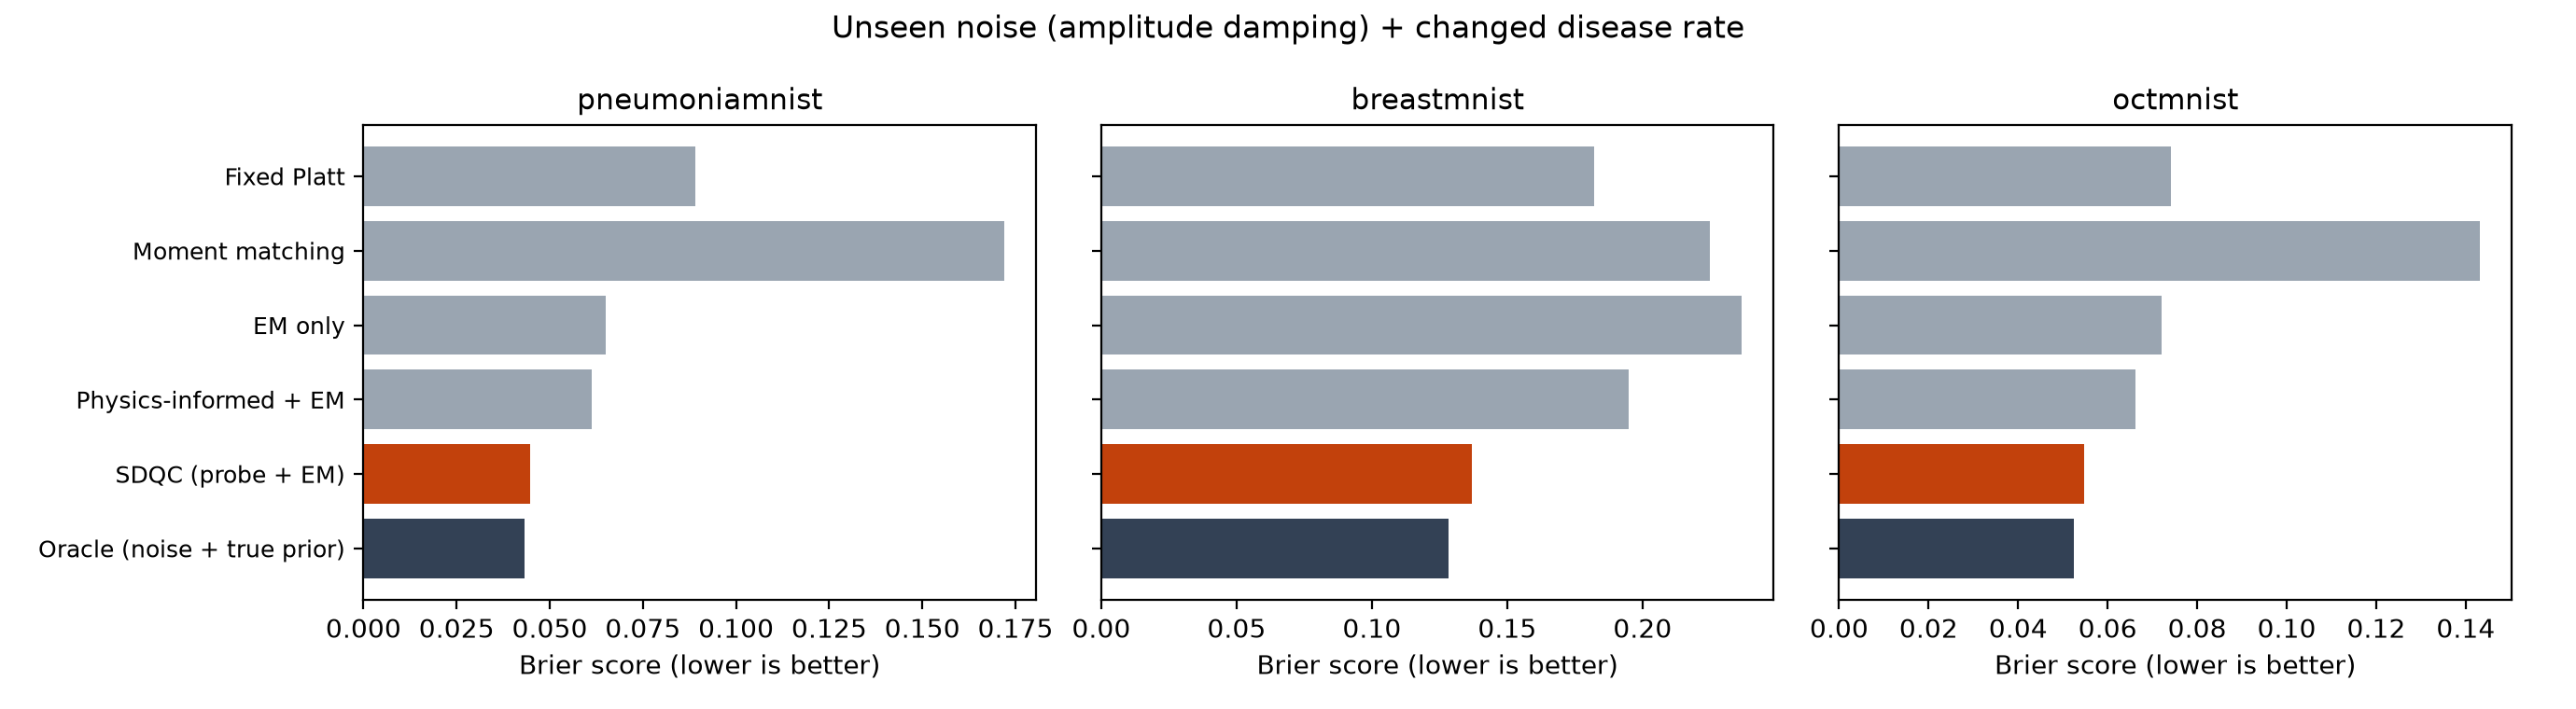
\includegraphics[width=0.95\textwidth]{hard_case.png}
\caption{Hard case (unseen amplitude damping, changed prevalence): mean Brier by method for each dataset (V5.1, 10 seeds). SDQC (orange) comes close to the oracle (dark) on all three datasets.}
\label{fig:hard}
\end{figure*}

Table~\ref{tab:hard_model} breaks the hard case down by model. SDQC improves on Fixed Platt, MM and Phys+EM for every model. The benefit is not specific to one architecture: it holds for the VQC, the re-uploading circuit and the kernel model.

\begin{table}[t]
\centering
\caption{Hard case by model: mean Brier (unseen amplitude damping, changed prevalence, 10 seeds).}
\label{tab:hard_model}
\setlength{\tabcolsep}{3.5pt}
\begin{adjustbox}{max width=\linewidth}
\begin{tabular}{llccccc}
\toprule
Dataset & Model & Fixed & MM & Phys+EM & SDQC & Oracle \\
\midrule
\multirow{2}{*}{Breast} & Re-upload & 0.1835 & 0.2229 & 0.1642 & \textbf{0.1304} & 0.1241 \\
 & VQC & 0.1808 & 0.2267 & 0.2197 & \textbf{0.1423} & 0.1314 \\
\midrule
\multirow{3}{*}{OCT} & QSVM & 0.0735 & 0.1365 & 0.0621 & \textbf{0.0570} & 0.0547 \\
 & Re-upload & 0.0767 & 0.1468 & 0.0809 & \textbf{0.0546} & 0.0524 \\
 & VQC & 0.0724 & 0.1460 & 0.0555 & \textbf{0.0525} & 0.0505 \\
\midrule
\multirow{3}{*}{Pneum.} & QSVM & 0.0889 & 0.1626 & 0.0593 & \textbf{0.0482} & 0.0466 \\
 & Re-upload & 0.0919 & 0.1760 & 0.0646 & \textbf{0.0440} & 0.0426 \\
 & VQC & 0.0862 & 0.1771 & 0.0600 & \textbf{0.0417} & 0.0404 \\
\bottomrule
\end{tabular}
\end{adjustbox}
\end{table}

Table~\ref{tab:byprior} breaks the PneumoniaMNIST hard case down by target prevalence. The largest gain is at $\pi_t=0.30$, the prevalence furthest from the source value of 0.74. There Fixed Platt scores 0.1288 and SDQC 0.0430. MM collapses at this prevalence (0.3030).

\begin{table*}[t]
\centering
\caption{PneumoniaMNIST hard case by target prevalence: mean Brier (10 seeds). $n$ is the test-subset size.}
\label{tab:byprior}
\begin{adjustbox}{max width=\linewidth}
\begin{tabular}{ccccccccc}
\toprule
$\pi_t$ & $n$ & Fixed & MM & EM only & Phys+EM & Probe only & SDQC & Oracle \\
\midrule
0.30 & 288 & 0.1288 & 0.3030 & 0.0643 & 0.0584 & 0.0775 & \textbf{0.0430} & 0.0408 \\
0.50 & 404 & 0.0994 & 0.1347 & 0.0822 & 0.0765 & 0.0666 & \textbf{0.0546} & 0.0536 \\
0.90 & 647 & 0.0388 & 0.0780 & 0.0485 & 0.0490 & 0.0422 & \textbf{0.0363} & 0.0352 \\
\bottomrule
\end{tabular}
\end{adjustbox}
\end{table*}

\subsection{Prevalence Estimation}

Table~\ref{tab:prior} shows \emph{why} SDQC works. Without drift correction, EM attributes the hardware change to a change in prevalence. On BreastMNIST its prevalence error rises from 0.054 (clean) to 0.231 (depolarizing) and 0.224 (amplitude damping). Correcting the scores with probes first brings the errors under noise back close to the clean level: 0.074 and 0.067 on BreastMNIST, and 0.041--0.049 on the larger datasets.

\begin{table}[t]
\centering
\caption{Mean absolute error of the estimated prevalence, changed-prevalence setting (10 seeds).}
\label{tab:prior}
\setlength{\tabcolsep}{3.5pt}
\begin{adjustbox}{max width=\linewidth}
\begin{tabular}{llcccc}
\toprule
Dataset & Hardware & EM only & Phys+EM & SDQC & SDQC-sim \\
\midrule
\multirow{3}{*}{Breast}
 & Clean  & 0.054 & 0.068 & 0.067 & 0.068 \\
 & Depol. & 0.231 & 0.100 & 0.074 & 0.074 \\
 & Amp.   & 0.224 & 0.167 & 0.067 & 0.068 \\
\midrule
\multirow{3}{*}{OCT}
 & Clean  & 0.044 & 0.040 & 0.039 & 0.040 \\
 & Depol. & 0.111 & 0.052 & 0.046 & 0.046 \\
 & Amp.   & 0.055 & 0.047 & 0.041 & 0.041 \\
\midrule
\multirow{3}{*}{Pneum.}
 & Clean  & 0.045 & 0.044 & 0.043 & 0.044 \\
 & Depol. & 0.099 & 0.053 & 0.049 & 0.050 \\
 & Amp.   & 0.068 & 0.070 & 0.046 & 0.046 \\
\bottomrule
\end{tabular}
\end{adjustbox}
\end{table}

\subsection{Probe Diagnostics}

Table~\ref{tab:probe} gives the average fitted slope and residual RMSE of the probe fits under noisy hardware. A slope of about 0.61 means that, on average, deployment hardware shrinks scores to about 61\% of their calibration-day spread. The simulator reference gives a lower slope (about 0.54), because it also absorbs the reference device's own noise into the map. The residual RMSE is not small, because 1,000-shot deployment scores are noisy. Even so, an affine map fitted on 96 points is enough to recover most of the calibration, and the two reference choices end up within 0.0003 Brier of each other (Table~\ref{tab:paired_changed}).

\begin{table}[t]
\centering
\caption{Probe-fit diagnostics (noisy conditions, 10 seeds): mean fitted slope $\hat a$ and residual RMSE.}
\label{tab:probe}
\begin{adjustbox}{max width=\linewidth}
\begin{tabular}{lcccc}
\toprule
 & \multicolumn{2}{c}{Hardware reference} & \multicolumn{2}{c}{Simulator reference} \\
\cmidrule(lr){2-3}\cmidrule(lr){4-5}
Dataset & Slope & RMSE & Slope & RMSE \\
\midrule
BreastMNIST    & 0.610 & 0.121 & 0.541 & 0.119 \\
OCTMNIST       & 0.612 & 0.265 & 0.548 & 0.261 \\
PneumoniaMNIST & 0.606 & 0.216 & 0.541 & 0.213 \\
\bottomrule
\end{tabular}
\end{adjustbox}
\end{table}

\subsection{Preliminary Ablation: Strong Joint Noise and Probe Budget}

\emph{This subsection reports an earlier, smaller study and should be read as preliminary.} It used one seed, the VQC only, 192 evaluation records and two probe-selection repeats, with an earlier SDQC version and a probe budget of 8 or 16 (not 96). It added a ``strong joint'' condition (strong depolarizing, amplitude damping and readout error together) and an ``unreported'' condition in which the device's error report is wrong. Tables~\ref{tab:pre_joint}--\ref{tab:pre_budget} report the results. The trends agree with the main study. SDQC's advantage grows as noise becomes stronger and less well reported (0.2329 to 0.1484 Brier under strong joint noise). It lowers the prevalence error from 0.343 (EM only) to 0.138. Doubling the probes from 8 to 16 lowers Brier from 0.0938 to 0.0663, and from 0.1891 to 0.1078 under strong joint noise. This suggests that, at small budgets, the number of probes matters. Because of the single seed, no confidence intervals are reported.

\begin{table}[t]
\centering
\caption{Preliminary (1 seed, VQC, 192 records): mean Brier by hardware condition.}
\label{tab:pre_joint}
\begin{adjustbox}{max width=\linewidth}
\begin{tabular}{lcccc}
\toprule
Condition & Fixed & EM only & Probe only & SDQC \\
\midrule
Clean        & 0.0544 & 0.0436 & 0.0530 & \textbf{0.0430} \\
Unreported   & 0.0962 & 0.0773 & 0.0615 & \textbf{0.0489} \\
Strong joint & 0.2329 & 0.3549 & \textbf{0.1452} & 0.1484 \\
\bottomrule
\end{tabular}
\end{adjustbox}
\end{table}

\begin{table}[t]
\centering
\caption{Preliminary (1 seed, VQC): mean Brier by target prevalence.}
\label{tab:pre_prior}
\begin{adjustbox}{max width=\linewidth}
\begin{tabular}{lcccc}
\toprule
$\pi_t$ & Fixed & EM only & Probe only & SDQC \\
\midrule
0.30   & 0.2107 & 0.2473 & 0.1226 & \textbf{0.0963} \\
0.50   & 0.1560 & 0.1952 & 0.1005 & \textbf{0.0972} \\
0.90   & 0.0529 & 0.0668 & 0.0534 & \textbf{0.0506} \\
Source & 0.0917 & 0.1252 & \textbf{0.0697} & 0.0763 \\
\bottomrule
\end{tabular}
\end{adjustbox}
\end{table}

\begin{table}[t]
\centering
\caption{Preliminary (1 seed, VQC): SDQC Brier by probe budget, and prevalence error under strong joint noise.}
\label{tab:pre_budget}
\begin{adjustbox}{max width=\linewidth}
\begin{tabular}{lcc}
\toprule
 & 8 probes & 16 probes \\
\midrule
SDQC Brier (all conditions)  & 0.0938 & 0.0663 \\
SDQC Brier (strong joint)    & 0.1891 & 0.1078 \\
\midrule
\multicolumn{3}{l}{Prevalence MAE, strong joint: EM only 0.343; SDQC 0.138} \\
\bottomrule
\end{tabular}
\end{adjustbox}
\end{table}

% ============================================================
\section{Discussion}

\textbf{Why SDQC works.} The probes break the confounding between hardware drift and label shift. Hardware drift changes $p(z\mid y)$, and that change is visible on fixed inputs. Label shift changes $p(y)$ only, and is invisible on fixed inputs. By correcting the drift first, SDQC returns the problem to the setting where EM is known to work well~\cite{alexandari2020}: a calibrated classifier with a fixed $p(z\mid y)$. This is why EM-only and MM, each of which handles one effect while ignoring the other, fail in opposite directions.

\textbf{Hardware versus simulator reference.} SDQC and SDQC-sim differ by at most 0.0003 Brier. In this simulation the reference hardware is only lightly noisy, so the simulator is a close stand-in. On real devices, where the reference noise is larger and harder to model, measuring the reference on hardware should matter more. SDQC with a hardware reference also needs no simulator at all, which is why we make it the default.

\textbf{When not to use EM.} Where prevalence is known to be stable, or the deployment batch is small (BreastMNIST), the EM step adds variance that probe-only correction avoids. A practical rule is to apply probe correction always and EM only when the batch is large or there is evidence of a change in prevalence. Shrinkage with $\lambda=0.85$ reduces this cost but does not remove it.

\textbf{Classical relevance.} The V4 classical control shows that the transfer problem comes from score distortion, not from anything specifically quantum. Probe-based drift correction could therefore apply to any classifier deployed on drifting hardware, including analog accelerators.

% ============================================================
\section{Limitations}

\begin{itemize}
\item \textbf{Simulated noise.} All noise is simulated with standard channels and affects every input in the same way. Real devices show crosstalk, non-Markovian drift and input-dependent errors that an affine map may not capture. Validation on real quantum hardware is the most important next step.
\item \textbf{Small BreastMNIST.} With 94 test images, results on BreastMNIST have high variance, and the EM step costs up to about 0.015 Brier when prevalence is unchanged.
\item \textbf{Kernel model.} The QSVM noise model perturbs kernel estimates as a proxy for hardware noise. It does not simulate the full kernel circuit on noisy hardware for every pair of inputs.
\item \textbf{Statistical scope.} Ten seeds but a single fixed data split per dataset. The bootstrap intervals capture variation across seeds, models and hardware conditions, but not variation across data splits. The V4 benchmark used three seeds.
\item \textbf{Low-dimensional features.} Four PCA features from a frozen ResNet-18 keep the circuits small. Most of the discriminative work is done by the classical extractor.
\item \textbf{Label shift only.} SDQC assumes that the class-conditional image distribution is unchanged. Covariate shift, such as images from a new scanner, is not addressed.
\item \textbf{Preliminary ablation.} The 8/16-probe and strong-joint-noise results come from a single-seed study of the VQC alone and need full replication.
\end{itemize}

% ============================================================
\section{Future Work}

Directions for further work include:
\begin{itemize}
\item running SDQC on IBM or IonQ hardware across several calibration cycles;
\item selecting probes adaptively, and modelling drift with non-affine (e.g., isotonic) response maps;
\item a test for whether prevalence has changed, to decide when to run EM;
\item extension to multi-class tasks;
\item combining SDQC with conformal prediction~\cite{park2024} to give coverage guarantees under drift.
\end{itemize}

% ============================================================
\section{Conclusion}

Noise on quantum hardware damages the calibration of hybrid medical image classifiers. That damage is easy to repair with labels from the current device and hard to repair without them, especially when patient prevalence may also have changed. SDQC separates the two effects using a small set of probe inputs measured on calibration day and at deployment. Across three MedMNIST tasks, three quantum models, 29 hardware conditions including unseen amplitude damping, four prevalences and ten seeds, it beat every deployable baseline whenever prevalence changed. In the hardest PneumoniaMNIST setting it reached 0.0446 Brier, against 0.0432 for an oracle that knows both the noise and the true prevalence. Its main cost, from EM when prevalence is stable on very small datasets, is reported openly and points to a simple practical rule.

% ============================================================
\begin{thebibliography}{00}

\bibitem{gupta2025} % TODO: verify against your existing .bib entry
R. Gupta \emph{et al.}, ``Quantum machine learning for medical image classification,'' 2025.

\bibitem{sunki2025} % TODO: verify chapter/book details
A. Sunki \emph{et al.}, ``Quantum computing applications in healthcare and medical imaging,'' book chapter, 2025.

\bibitem{guo2017}
C. Guo, G. Pleiss, Y. Sun, and K. Q. Weinberger, ``On calibration of modern neural networks,'' in \emph{Proc. ICML}, 2017, pp. 1321--1330.

\bibitem{ovadia2019}
Y. Ovadia \emph{et al.}, ``Can you trust your model's uncertainty? Evaluating predictive uncertainty under dataset shift,'' in \emph{Proc. NeurIPS}, 2019.

\bibitem{platt1999}
J. Platt, ``Probabilistic outputs for support vector machines and comparisons to regularized likelihood methods,'' in \emph{Advances in Large Margin Classifiers}, MIT Press, 1999, pp. 61--74.

\bibitem{zadrozny2002}
B. Zadrozny and C. Elkan, ``Transforming classifier scores into accurate multiclass probability estimates,'' in \emph{Proc. ACM SIGKDD}, 2002, pp. 694--699.

\bibitem{niculescu2005}
A. Niculescu-Mizil and R. Caruana, ``Predicting good probabilities with supervised learning,'' in \emph{Proc. ICML}, 2005, pp. 625--632.

\bibitem{saerens2002}
M. Saerens, P. Latinne, and C. Decaestecker, ``Adjusting the outputs of a classifier to new a priori probabilities: A simple procedure,'' \emph{Neural Computation}, vol. 14, no. 1, pp. 21--41, 2002.

\bibitem{lipton2018}
Z. C. Lipton, Y.-X. Wang, and A. Smola, ``Detecting and correcting for label shift with black box predictors,'' in \emph{Proc. ICML}, 2018.

\bibitem{alexandari2020}
A. Alexandari, A. Kundaje, and A. Shrikumar, ``Maximum likelihood with bias-corrected calibration is hard-to-beat at label shift adaptation,'' in \emph{Proc. ICML}, 2020.

\bibitem{yang2023}
J. Yang \emph{et al.}, ``MedMNIST v2: A large-scale lightweight benchmark for 2D and 3D biomedical image classification,'' \emph{Scientific Data}, vol. 10, no. 41, 2023.

\bibitem{he2016}
K. He, X. Zhang, S. Ren, and J. Sun, ``Deep residual learning for image recognition,'' in \emph{Proc. IEEE CVPR}, 2016, pp. 770--778.

\bibitem{preskill2018}
J. Preskill, ``Quantum computing in the NISQ era and beyond,'' \emph{Quantum}, vol. 2, p. 79, 2018.

\bibitem{schuld2020}
M. Schuld, A. Bocharov, K. M. Svore, and N. Wiebe, ``Circuit-centric quantum classifiers,'' \emph{Physical Review A}, vol. 101, 032308, 2020.

\bibitem{perez2020}
A. P\'erez-Salinas, A. Cervera-Lierta, E. Gil-Fuster, and J. I. Latorre, ``Data re-uploading for a universal quantum classifier,'' \emph{Quantum}, vol. 4, p. 226, 2020.

\bibitem{havlicek2019}
V. Havl\'i\v{c}ek \emph{et al.}, ``Supervised learning with quantum-enhanced feature spaces,'' \emph{Nature}, vol. 567, pp. 209--212, 2019.

\bibitem{bergholm2018}
V. Bergholm \emph{et al.}, ``PennyLane: Automatic differentiation of hybrid quantum-classical computations,'' arXiv:1811.04968, 2018.

\bibitem{bowles2024}
J. Bowles, S. Ahmed, and M. Schuld, ``Better than classical? The subtle art of benchmarking quantum machine learning models,'' arXiv:2403.07059, 2024.

\bibitem{park2024} % TODO: verify against your existing .bib entry
S. Park and O. Simeone, ``Quantum conformal prediction for reliable uncertainty quantification in quantum machine learning,'' \emph{IEEE Trans. Quantum Engineering}, 2024.

\bibitem{catak2025} % TODO: verify title/venue
F. O. Catak \emph{et al.}, ``Uncertainty quantification in quantum machine learning classifiers,'' 2025.

\bibitem{wendlinger2025} % TODO: verify title/venue
M. Wendlinger \emph{et al.}, ``Uncertainty and calibration of quantum neural networks,'' 2025.

\bibitem{spencer2026} % TODO: verify title/venue (AQCP)
Spencer \emph{et al.}, ``Adaptive quantum calibration (AQCP),'' 2026.

\end{thebibliography}

\end{document}
